\chapter{Background}
\label{chap:background}

\section{Introduction}

This chapter provides a brief and non-exhaustive overview of the theory and techniques used in this thesis.

First Section~\ref{subsec:background-terminology} defines terminology. Then Section~\ref{subsec:background-machine-learning} provides an overview of the machine learning techniques used in this thesis. Section~\ref{subsec:background-gpgpu} provides an overview of GPGPU programming. % Section~\ref{subsec:background-statistics} describes the statistical tools and methodologies used in this thesis.
Lastly Section~\ref{subsec:background-summary} concludes.


\section{Terminology}
\label{subsec:background-terminology}

\emph{Machine learning} refers to a family of statistical models and algorithms used to \emph{infer} a function for future values given past example values.

\emph{Deep learning} is a loosely defined class of machine learning methods built on artificial neural networks. It is often confused with \emph{deep neural networks}, which are simply artificial neural networks with one or more hidden layers. In this thesis, \emph{deep learning} is used to describe Recurrent Neural Networks.

% \emph{feature space}

% \emph{supervised learning}

% \emph{unsupervised learning}


\section{Machine Learning}
\label{subsec:background-machine-learning}

Machine learning techniques are used in this thesis for classification and sequential modelling. Classification is the task of predicting the correct category --- or class --- for a new instance, based on ``labelled'' training data, i.e.\ instances whose categories are known. The properties describing instances are called \emph{features}. Sequence modelling is the task of capturing the underling probability distribution describing a sequence of values. This section briefly describes the classification and sequential modelling techniques used in this thesis.


\subsection{ZeroR}

A ``ZeroR'' classifier is a model whose output is always the mode of the training data classes, irrespective of the input features. For example, given training data with the labels $\left( A B B C \right)$, the model will predict $B$ for all future values. A ZeroR model represents the simplest approach to classification, and is useful for providing a baseline to evaluate the performance of more complex classifiers, since a ZeroR classifier has no power of prediction.


\subsection{Decision Trees}

Decision trees are an intuitive form of classifier in which a tree structure of decision nodes are used to predict the class for a given set of features. Decision trees are built using binary recursive partitioning: by creating a decision node for the feature which provides the highest gain, creating new child nodes for each possible outcome, splitting dividing the data amongst these child nodes, and continuing recursively. To find the gain of an feature, we first compute the entropy of the data set. Given a set of data points $D$, and $p_{(+)}$ and $p_{(-)}$ are the number of positive and negative examples in $D$:

\begin{equation}
  H(D) = - p_{(+)}\log_2p_{(+)} - p_{(-)}\log_2p_{(-)}
\end{equation}

The gain of a feature $x$ is found using:

\begin{equation}
  \gain(D, x) = H(D) - \sum_{V \in \text{Values}(x)}\frac{|D_V|}{|D|}H(D_V)
\end{equation}

Decision trees are popular and low overhead form of classification, as implementations can be as simple and efficient as a nested set of \texttt{if}/\texttt{else} statements. However, care must be taken to avoid over-fitting to training data.


\subsection{Artificial Neural Networks}

Artificial Neural Networks can be used when non-linearity is desired. They use a network of neurons to map the input variables to a response or prediction. Each neuron in the network is connected by weighted edges, as can be seen in Figure~\ref{fig:} which represents a typical feed-forward multi-layered neural networks.

Feed-forward

In common ANN implementations, the signal at a connection between artificial neurons is a real number, and the output of each artificial neuron is computed by some non-linear function of the sum of its inputs. The connections between artificial neurons are called 'edges'. Artificial neurons and edges typically have a weight that adjusts as learning proceeds.

\begin{figure}
  \centering
  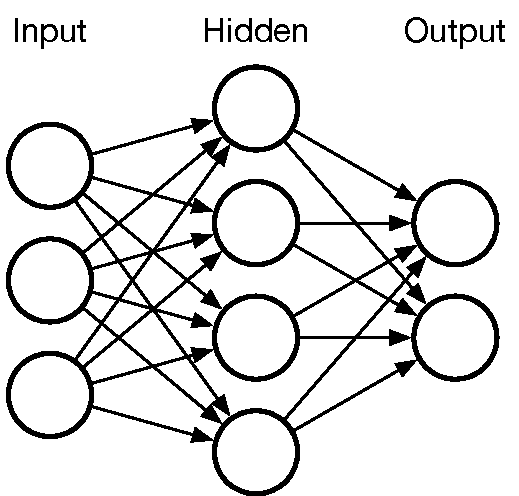
\includegraphics[width=.45\columnwidth]{img/artificial-neural-network}%
  \caption[Structure of an artificial neural network]{%
    The anatomy of an artificial neural network. This graph representation uses nodes to represent artificial neurons, and edges to represent the output of one neuron into the input of another.%
  }%
  \label{fig:artificial-neural-network}
\end{figure}


\subsection{Recurrent Neural Networks}

A recurrent neural network (RNN) consists of hidden states \textbf{h} an an optional output \textbf{y}. It operates on a variable-length sequence, $\bm{x} = \left( x_1, x_2, \ldots, x_T \right)$. At each step $t \in T$, the hideen state $h_{<t>}$ of the RNN is updated by:

\[ h_{<t>} = f\left( h_{<t-1>}, x_t \right) \]

where $f$ is a non-linear activation function. An RNN can learn a probabilty distribution over a sequence of tokens to predict the next token. Therefore, at each timestep $t$, the output from the RNN is a conditional distribution $p\left( x_t | x_1, \ldots, x_{t-1} \right)$.

% De Boom, C., Dhoedt, B., & Demeester, T. (2018). Character-level Recurrent Neural Networks in Practice: Comparing Training and Sampling Schemes. ArXiv:1801.00632.
\todo[inline]{RNN evaluation~\cite{DeBoom2018}.}

\subsection{Long Short-Term Memory}

The long short-term memory (LSTM) is an RNN architecture.

LSTM variants review~\cite{Greff2015}.

$\bm{x}^t$ is the input vector at time $t$; $\bm{W}$ are input weight matrices; $\bm{R}$ are recurrent weight matrices; $\bm{p}$ are peephole weight vectors; $\bm{b}$ are bias vectors; functions $g$, $h$, and $\sigma$ are point-wise nonlinear activation functions.

block input:
\[ \bm{z}^{t} = g \left( \bm{W}_z \bm{x}^t + \bm{R}_z \bm{y}^{t - 1} + \bm{b}_z \right) \]

input gate:
\[ \bm{i}^{t} = \sigma \left( \bm{W}_i \bm{x}^t + \bm{R}_i \bm{y}^{t-1} + \bm{p}_i \odot c^{t-1} + \bm{b}_i \right) \]

forget gate:
\[ \bm{f}^{t} = \sigma \left( \bm{W}_f \bm{x}^t + \bm{R}_f \bm{y}^{t-1} + \bm{p}_f \odot c^{t-1} + \bm{b}_f \right) \]

cell state:
\[ \bm{c}^t = \bm{i}^t \odot \bm{z}^t + \bm{f}^t \odot \bm{c}^{t-1} \]

output gate:
\[ \bm{o}^{t} = \sigma \left( \bm{W}_i \bm{x}^t + \bm{R}_o \bm{y}^{t - 1} + \bm{p}_o \odot c^{t-1} + \bm{b}_o \right) \]

block output:
\[ \bm{y}^t = \bm{o}^t \odot h(\bm{c}^t) \]

Number of params = \todo[inline]{\ldots}


% TODO: \subsection{Generative Adversarial Networks}

The Generative Adversarial Network (GAN) is a means to estimate a generative model~\cite{Goodfellow2014}. It uses an adversarial process in which two models are simultaneously trained: a generator model $G$ that captures the data distribution, and a discriminative model $D$ that estimates the probability that a sample came from the training data rather than $G$. The training procedure for $G$ is to maximise the probability of $D$ making a mistake.

If both models are neural networks: learn a generator's distribution $p_g$ over data $\bm{x}$. Define a prior on input noise variables $p_z(\bm{z})$. Generator $G(\bm{z}; \Theta_g)$, using parameters $\Theta_g$. Discriminator $D(\bm{x}; \Theta_d)$ outputs a scalar, the probability that $\bm{x}$ came from the data rather than $p_g$.

Simultaneously train $D$ to maximise the probability of assigning the correct label to both training examples and samples from $G$, and train $G$ to minimise $\log (1 - D(G(\bm{z})))$. $D$ and $G$ play the two-player minimax game with value function $V(G, D)$:

\[ \min_G \max_D V(D, G) = \mathbb{E}_{\bm{x} \sim  p_{data}(\bm{x})} [ \log D(\bm{x}) ] + \mathbb{E}_{\bm{z} \sim p_z(\bm{z})} [ \log (1 - D(G(\bm{z}))) ] \]

Challenge: there may not be sufficient gradient for $G$ to learn well. Early in learning, when $G$ is poor, $D$ can reject samples with high confidence because they are clearly different from the training data.


\section{GPGPU Programming}
\label{subsec:background-gpgpu}

General purpose programming with graphics hardware is a nascent field, but has shown to enable massive data parallel throughput by re-purposing the hardware traditionally dedicated to the rendering of 3D graphics for generic computation. This was enabled by hardware support for programmable shaders replacing the fixed function graphics pipeline, and support for floating point operations in 2001. \citeauthor{Owens2006} provide a review of the first five years of general purpose computation on graphics hardware in~\cite{Owens2006}.

In the ensuing progress towards increasingly programmable graphics hardware, two dominant programming models have emerged: CUDA and OpenCL, which both abstract the graphics primitives of GPU hardware and provide a platform for GPGPU programming. CUDA is a language developed by NVIDIA for programming their GPUs using a proprietary SDK and API~\cite{Nvidia2007}, while OpenCL is a vendor-independent open standard based on a subset of the ISO C99 programming language, with implementations for devices from most major GPU manufactures~\cite{Stone2010}. Quantitative evaluations of the performance of CUDA and OpenCL programs suggest that performance is comparable between the two systems, although the wider range of target architectures for OpenCL means that appropriate optimisations must be made by hand or by the compiler~\cite{Komatsu2010,Karimi2010}.

\subsection{The OpenCL Programming Model}

OpenCL is a parallel programming framework which targets CPUs, GPUs, and other parallel processors such as Field-Programmable Gate Arrays. It provides a set of APIs and a language (based on an extended subset of C) for controlling heterogeneous \emph{compute devices} from a central host. Programs written for these devices are called \emph{kernels}, and are compiled by platform-specific tool chains. At runtime, an OpenCL \emph{platform} is selected and a \emph{context} object is created which exposes access to each supported compute device through \emph{command queues}. When a kernel is executed, each unit of computation is referred to as a \emph{work-item}, and these work-items are grouped into \emph{work-groups}. The sum of all work-group dimensions defines the \emph{global size}. For GPUs, work-groups execute on the Single Instruction Multiple Data (SIMD) processing units in lockstep. This is very different from the behaviour of traditional CPUs, and can cause severe performance penalties in the presence of flow control, as work-items must be stalled across divering flow paths.


\subsubsection{Memory Model}

Unlike the flat model of CPUs, OpenCL uses a hierarchical memory model, shown in Figure~\ref{fig:opencl-memory}. The host and each OpenCL device has a single global memory address space. Each work-group has a local memory space, and each work-item has a region of private memory.

Work-groups cannot access the memory of neighbouring work-groups, nor can work-items access the private memory of other work-items. OpenCL provides synchronisation barriers to allow for communication between work-items within a single work-group via the local memory, but not global barriers. Memory transfers between the host and devices occurs between global memory regions. In the case of programming heterogeneous devices, these transfers must occur over the connection bus between the CPU and device (e.g.\ PCIe for discrete GPUs), which typically creates a performance bottleneck by introducing a performance overhead to transfer data to the device for processing, then back to the device afterwards. Direct transfers of data between devices is not supported, requiring an intermediate transfer to the host memory.

\begin{figure}
	\centering
	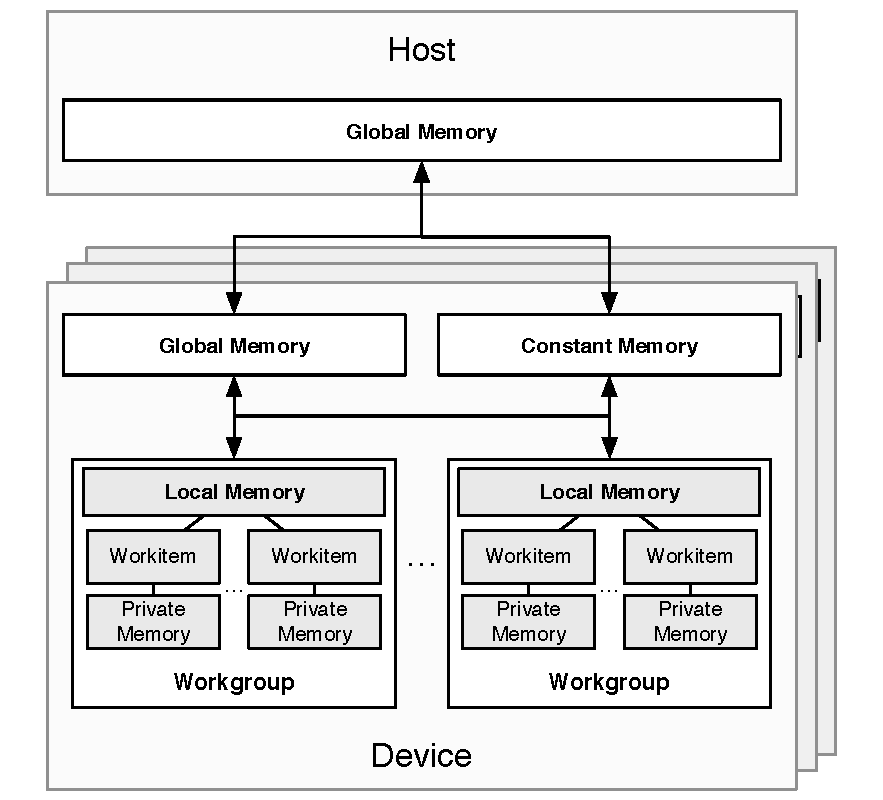
\includegraphics[width=0.8\textwidth]{img/opencl-memory}
	\caption[The OpenCL memory model]{%
		The OpenCL memory model. The host communicates with each device through transfers between global memory spaces. The capacity of each type of memory is dependent on the device hardware. In general, private memory is the fastest and smallest, and global memory is the largest and slowest.%
	}
	\label{fig:opencl-memory}
\end{figure}

\subsubsection{Performance Optimisations}

The wide range of supported execution devices and differing standards-compliant implementations makes portable performance tuning of OpenCL programs a difficult task~\cite{Rul2010}, and the interactions between optimisations and the hardware are complex and sometimes counter-intuitive~\cite{Ryoo2008}.

The overhead introduced by memory transfers between host and compute devices further complicates comparisons of OpenCL performance on different devices. The conclusion of~\cite{Gregg2011} is that this overhead can account for a $2\times$ to $50\times$ difference of GPU program runtime. In~\cite{Lee2010}, \citeauthor{Lee2010} present a performance analysis of optimised throughput computing applications for GPUs and CPUs. Of the 14 applications tested, they found GPU performance to be $0.7\times$ to $14.9\times$ that of multi-threaded CPU code, with an average of only 2.5$\times$. This is much lower than the $100\times$ to $1000\times$ values reported by other studies, a fact that they attribute to uneven comparison of optimised GPU code to unoptimised CPU code, or vice versa. \citeauthor{Lee2010} found that multi-threading, cache blocking, reordering of memory accesses and use of SIMD instructions to contribute most to CPU performance. For GPUs, the most effective optimisations are reducing synchronisation costs, and exploiting local shared memory. In all cases, the programs were optimised and hand-tuned by programmers with expert knowledge of the target architectures. It is unclear whether their performance results still hold for subsequent generations of devices.

Despite the concerns of over-represented speedups, the potential for high performance coupled with the complexity and low levels of abstraction provided by OpenCL make it an ideal target for skeletal abstractions. SkelCL and SkePU are two such examples which add a layer of abstraction above OpenCL and CUDA respectively in order to simplify GPGPU programming~\cite{Enmyren2010}.


% \subsection{Evaluation Techniques}
% \label{subsec:background-statistics}

% This section describes a number of the statistical tools and evaluation techniques used throughout this thesis.


% \subsubsection{Interquartile Range}

% Quartiles are the three points that divide an ordered set of data values into four groups of equal size. The first quartile $Q_1$ is the point which divides the data equally between the lowest value and the median, $Q_2$. The third quartile $Q_3$ is the point which divides the data between the median and the highest value. The interquartile range (IQR) measures the dispersion of a data set, and is the difference between the third and first quartiles, $Q_3 - Q_1$.


% \subsubsection{Confidence Intervals}

% Confidence intervals estimate the interval for the true range of a population parameter. Given a set of samples of a population with estimates of a parameter value for each, the confidence interval $(c_1,c_2)$ estimates the frequency that the true parameter value will fall between the per-sample confidence interval. Given a sample $x$ with sample size $n$, the confidence interval for a confidence $\alpha$ is found using:

% \begin{align}
%   \bar{x} &= \frac{1}{n}\sum_{i=1}^{n} x_i\\
%   \sigma &= \sqrt{\frac{\sum_{i=1}^{n}(x_i - \bar{x})^2}{n - 1}}\\
%   c_1 &= \bar{x} - z_{1-\alpha/2}\frac{\sigma}{\sqrt{n}}\\
%   c_2 &= \bar{x} + z_{1-\alpha/2}\frac{\sigma}{\sqrt{n}}
% \end{align}

% Where the value $z_{1-\alpha/2}$ assumes a Gaussian distribution of
% the underlying data, and the values for popular $\alpha$ values are
% typically found using pre-computed ``Z-tables''. To calculate
% confidence intervals for the ratio of two means, $\bar{x}_1$ and
% $\bar{x}_2$ with sample sizes $n_1$ and $n_2$, and respective standard
% deviations $\sigma_1$ and $\sigma_2$:

% \begin{align}
%   \sigma_x &= \sqrt{\frac{\sigma_1^2}{n_1} + \frac{\sigma_2^2}{n_2}}\\
%   c_1 &= \bar{x}_1 - \bar{x}_2 - z_{1-\alpha/2}\sigma_x\\
%   c_2 &= \bar{x}_1 - \bar{x}_2 + z_{1-\alpha/2}\sigma_x
% \end{align}

% The above calculations assumes that the sample variance ($\sigma^2$)
% is an accurate estimation of the true population variance. This relies
% on the assumption of an underlying Gaussian distribution, which,
% according to the central limit theorem, is true of large sample sizes
% (typically $n \ge 30$). In cases of smaller sample sizes, the sample
% and population variances can differ significantly, so one must instead
% use a Student's $t$-distribution, $t_{1-\alpha/2}$, in place of
% $z_{1-\alpha/2}$.


% \subsubsection{Histogram}

% Histograms show the distribution of numerical data. The data is first divided into a set of discrete, equally sized sub-intervals, or \emph{bins}. The number of data points in each bin is used to show visualise the density distribution. The shortcoming of histograms is that their appearance is heavily influenced by three user-selected parameters: the number of bins, the width of bins, and the endpoints chosen. As such, they may provide a misleading representation of the data if inappropriate values for any of these parameters are chosen. Kernel Density estimation is a technique for showing the distribution of data which circumvents some of these issues.

% \subsubsection{Kernel Density Estimation}

% A Kernel Density Estimate (KDE) is an approximation of the probability
% density function of a random variable. Given a random variable $x$,
% and bandwidth $h$ and a kernel $K$, the Kernel Density Estimate
% $\hat{f}_h(x)$ can be found using:
% %
% \begin{equation}
%   \hat{f}_h(x) = \frac{1}{nh} \sum^{n}_{i=1} K\left( \frac{x - x_i}{h} \right)
% \end{equation}
% %
% Using a smooth kernel such as a Gaussian distribution for the kernel
% produces a smooth density estimated, unlike histograms. However, like
% histograms, the appearance of a Kernel Density Estimate plot is
% dependent on the value of the bandwidth parameter $h$ (equivalent to
% binwidth in histograms), so care must be taken to select a value to
% minimise over or under smoothing. Grouped data can be shown by
% plotting multiple KDEs on the same axes, although if the number of
% groups is large, a box plot or violin plot may be more appropriate.


% \subsubsection{Box plot}

% Box plots are used to show the distribution of quartile ranges for
% grouped data. The contain the following features:
% %
% \begin{itemize}
%   \item Horizontal lines at the lower quartile, median and upper
%   quartile.
%   \item Vertical lines above and below the upper and lower quartiles to
%   the most extreme data point within 1.5 IQR of the upper/lower
%   quartile, with horizontal whiskers at the end of the vertical lines.
%   \item Dots beyond the ends of the vertical lines to show outliers.
% \end{itemize}
% %
% A variation of box plots used in this thesis is the violin plot, which
% extends the box plot with a fitted Kernel Density Estimate plot to
% show the probability \emph{density} of data at different values. To
% construct a violin plot, KDEs for each group are rotated and mirrored
% to generate a smoothed visualisation of the distribution.


\section{Differential Testing}

\todo[inline]{Difftesting overview, including the figure from the litreview.}


\section{Summary}
\label{subsec:background-summary}

This chapter details the machine learning techniques used in this thesis, and describes the domain for which they are applied, GPGPU programming. The following chapter surveys the research literature relevant to this work.
